\documentclass{beamer}

\usepackage{graphicx,helvet,textpos,times,verbatim,tikz,enumerate,url}%
\usepackage{wrapfig}
\usepackage{color}
\usepackage{extarrows,amsmath}
\usetheme{metropolis}           % Use metropolis theme

%=================================
%below for the tikz
\usepackage{amsfonts,mathrsfs,pifont,bbding,pgfpages}
\usepackage[latin1]{inputenc}%
\usepackage[normalem]{ulem}
\usepackage{MnSymbol,wasysym}

% TikZ styles for drawing
\usetikzlibrary{intersections}
\usetikzlibrary{arrows,shapes,shadows,positioning,automata,patterns}
\usetikzlibrary{trees,snakes,decorations.pathmorphing,decorations.markings}
\usetikzlibrary{shapes.geometric,backgrounds,calc}

% TikZ styles for drawing
\tikzstyle{block} = [draw,rectangle,rounded corners,thick,minimum height=2em,minimum width=2em,fill=blue!20,draw=black!40]
\tikzstyle{block0} = [draw,rectangle,rounded corners,thick,minimum height=2em,minimum width=2em,fill=white!20,draw=white!90]
\tikzstyle{blockr} = [draw,rectangle,rounded corners,thick,rounded corners=6,thick,minimum height=2em,minimum width=2em,black!90,fill=gray!30]
\tikzstyle{sum} = [draw,circle,inner sep=0mm,minimum size=5mm,thick,fill=gray!40]
\tikzstyle{connector} = [->,thick]
\tikzstyle{blockex} = [draw,rectangle,rounded corners,thick,minimum height=2em,minimum width=2em,thick,fill=gray!20]
\tikzstyle{blockexg} = [draw,rectangle,rounded corners,thick,minimum height=2em,minimum width=2em,thick,fill=gray!20]
\tikzstyle{line} = [thick]
\tikzstyle{branch} = [circle,inner sep=0pt,minimum size=1mm,fill=black,draw=black,black]
\tikzstyle{branch2} = [circle,inner sep=0pt,minimum size=1mm,fill=black,draw=black]
\tikzstyle{guide} = [thick]
\tikzstyle{snakeline} = [connector, decorate, decoration={pre length=0.2cm,
                         post length=0.2cm, snake, amplitude=.4mm,
                         segment length=2mm},thick, ->]
\tikzstyle{place}=[circle,thick,draw=black!75,fill=gray!20,minimum size=6mm]%

\renewcommand{\vec}[1]{\ensuremath{\boldsymbol{#1}}} % bold vectors
\def \myneq {\skew{-2}\not =} % \neq alone skews the dash
\newtheorem{myLemma}{Lemma}[section]



\title{Applied Nonlinear Control \\
        \large Chapter 6 ~-~ Feedback Linearization}
\author{\large Shuai Qian}
\date{\today}
\institute{School of Automation \\
        Nanjing University of Science and Technology}
        
%insert the page number and the total number in footline
\setbeamertemplate{footline}[frame number]
         
\begin{document}
  \maketitle

%contents---------------------------
  \begin{frame}
  \addtocounter{framenumber}{-2}
  \frametitle{Table of Contents}
  \thispagestyle{empty}
  \tableofcontents
  \end{frame}


  \section{1. Introduction}

  \begin{frame}{Introduction}
    \textbf{Central ideal of feedback linearization}
    \begin{itemize}
      \item Algebraically transform a nonlinear system dynamics into a (fully or partly) linear one, so that linear control techniques can be applied.
    \end{itemize}

    \textbf{Differences between feedback linearization and conventional linearization}
    \begin{itemize}
      \item \textcolor{red}{Feedback linearization} : achieved by exact state transformations and feedback.
      \item \textcolor{red}{Conventional linearization} (Jacobian linearization) : linear approximations of the dynamics.
    \end{itemize}
   \end{frame}


   \begin{frame}{Jacobian Linearization}

    Consider a nonlinear autonomous system (\ref{nonlinear})
    \begin{equation}\label{nonlinear}
      \dot{\vec{x}} = \vec{f(x)}
    \end{equation}
    Assume that $\vec{f(x)}$ is continuously differentiable,
    then the system can be written as
    $$
    \dot{\vec{x}} = (\frac{\partial \vec{f}}{\partial \vec{x}})_{\vec{x}=0} + \vec{f}_{h.o.t.}(\vec{x})
    $$
    (0 is an equilibrium point, and $\vec{f}(0) = 0$).
    Let $\vec{A}$ denotes the Jacobian matrix of $\vec{f}$ with respect to $\vec{x}$ at $\vec{x}=0$
    $$
    \vec{A} = (\frac{\partial \vec{f}}{\partial \vec{x}})_{\vec{x}=0}
    $$
    Then, the system
    $$
    \dot{\vec{x}} = \vec{Ax}
    $$
   \end{frame}


%---------------------------------
  \section{2. Intuitive Concepts}

  \begin{frame}{Example}
    Consider the control of the level $h$ of fluid in a tank (Figure \ref{tank}) to a specified level $h_{d}$.

    %place the figure and word together!
    \begin{wrapfigure}{l}{4cm}
    \vspace{-10pt}
    \includegraphics[width=4cm]{image/tank.pdf}\\
    \vspace{-15pt}
    \caption{Fluid level control in a tank}\label{tank}
    \vspace{-10pt}
    \end{wrapfigure}

    Variables:
    \begin{itemize}
      \item Control input : $u$
      \item Cross section of the tank : $A(h)$
      \item Cross section of the outlet \\ pipe : $a$
      \item Desired level : $h_{d}$
    \end{itemize}

    The dynamic model of the tank is
    \begin{equation}\label{dynamic}
      \frac{d}{dt}\left[\int_{0}^{h}A(h)dh\right] = u(t) - a \sqrt{2gh}
    \end{equation}

  \end{frame}


  \begin{frame}{Feedback Linearization}
  The dynamic (\ref{dynamic}) can be rewritten as
  $$ A(h)\dot{h} = u-a\sqrt{2gh} $$
  If we choose $u(t)$ as
  $$
  Origin~dynamic \quad \xrightarrow[linearization]{{\color{red} u(t) = a\sqrt{2gh} + A(h)v}} \quad \dot{h}=v
  $$

  with $v$ being an \textbf{``equivalent input"} to be specified.
  Choosing $v$ as
  $$
   \dot{h}=v \quad \xrightarrow[close-loop]{{\color{red} v=-\alpha \widetilde{h}}} \quad \dot{h}+\alpha \widetilde{h}=0
  $$
  with $\widetilde{h} = h(t)-h_{d}$ being the \textbf{level error} ($\widetilde{h}(t)\rightarrow 0 ~\text{as}~ t \rightarrow \infty$), and $\alpha$ being a strictly positive constant.
  \end{frame}


  \begin{frame}{Feedback Linearization, ctd'}
  Finally, the actual input flow is determined by the nonlinear control law
  $$ u(t) = a\sqrt{2gh} - A(h)\alpha \widetilde{h} $$
    The idea of canceling the nonlinearities and imposing a desired linear dynamics, can be simply applied to a class of nonlinear systems described by the so-called \textbf{companion form, or controllability canonical form}:
    \begin{equation}\label{companion}
      x^{(n)} = f(\textbf{x}) + b(\textbf{x})u
    \end{equation}
    \vspace{-15pt}
    \begin{itemize}
      \item $u$ : scalar control input
      \item $x$ : scalar output of interest
      \item $\textbf{x} = \left[ x,\dot{x},\dots,x^{(n-1)}\right]^{T}$ : state vector
      \item $f(\textbf{x}), b(\textbf{x})$ : nonlinear functions of the states
    \end{itemize}
  \end{frame}


  \begin{frame}{Feedback Linearization, ctd'}
  In state-space representation, (\ref{companion}) can be written
  $$
  \frac{d}{dt}\left[\begin{array}{c}
                      x_{1} \\
                      \dots \\
                      x_{n-1} \\
                      x_{n}
                    \end{array}\right] = \left[\begin{array}{c}
                                                 x_{2} \\
                                                 \dots \\
                                                 x_{n} \\
                                                 f(\textbf{x}+b(\textbf{x})u)
                                               \end{array}\right]
  $$
  Using the control input ($b \neq 0$)\footnote{In our example, $b=\frac{1}{A(h)}, ~ f=-\frac{a\sqrt{2gh}}{A(h)}$}

  \begin{equation}\label{input}
    u = \frac{1}{b}\left[v-f\right]
  \end{equation}
  %(in example, $b=\frac{1}{A(h)}, ~ f=-\frac{a\sqrt{2gh}}{A(h)}$) \\
  we can cancel the nonlinearities and obtain the simple input-output relation
  $$ x^{(n)} = f(\textbf{x}) + b(\textbf{x})u \quad \xrightarrow[linearization]{E.q.(\ref{input})} \quad x^{(n)} = v $$
  \end{frame}


  \begin{frame}{Feedback Linearization, ctd'}
    Thus, the control law
    $$ v = -k_{0}x-k_{1}\dot{x}- \dots - k_{n-1}x^{(n-1)} $$
    with the $k_{i}$ chosen so that the polynomial $p^{n}+k_{n-1}p^{n-1} + \dots + k_{0}$ has all its roots strictly in the left-half complex plane, leads to the exponentially stable dynamics
    $$
    x^{n}+k_{n-1}x^{n-1}+\dots+k_{0}x = 0
    $$
    which implies that $x(t) \rightarrow 0$.
  \end{frame}

  \begin{frame}{Feedback Linearization, ctd'}
    For tasks involving the tracking of a desired output $x_{d}(t)$, the control law
    \begin{equation}\label{tracking}
      v = x_{d}^{(n)} - k_{0}e - k_{1}\dot{e}-\dots-k_{n-1}e^{(n-1)}
    \end{equation}
    where $e(t) = x(t)-x_{d}(t)$ is the tracking error, the control law leads to exponentially convergent tracking.
    \par \vspace{-5pt}
    \textcolor{red}{In our example}, $x_{d}(t)=h_{d}$ is constant, so choose
    $$v=-\alpha(h(t) - h_{d})$$
    with the $\alpha$ leads to the exponentially stable dynamics
    $$
    \dot{x} + \alpha x=0
    $$
    that is the polynomial $p+\alpha=0$ has all its roots strictly in the left-half complex plane
    $$
    p = -\alpha \quad \xrightarrow{p < 0} \quad \alpha > 0
    $$

  \end{frame}


  %=================================================================
  \section{3. Input-State Linearization}

  \begin{frame}{Input-State Linearization}
    Consider the single-input nonlinear system
    $$ \dot{x} = f(x,u) $$
    The technique of \textbf{input-state linearization} solves this problem in two steps :
    \begin{enumerate}
      \item Find a \textbf{state transformation} $z=z(x)$, and an \textbf{input transformation} $u=u(x,v)$ :
          $$ \dot{x} = f(x,u) \quad \xrightarrow[u=u(x,v)]{z=z(x)} \quad \underbrace{\dot{z}=Az+bv}_{{\color{red}LTI}} $$
      \item Uses standard linear techniques (such as pole placement) to design $v$.
    \end{enumerate}
  \end{frame}


  \begin{frame}{Example}
  Consider the system with the equilibrium point $(0, 0)$

  \begin{equation}\label{input-state-example}
  \begin{aligned}
    \dot{x}_{1} &= -2x_{1}+ax_{2}+\underbrace{\sin x_{1}}_{nonlinearity} \\
    \dot{x}_{2} &= \underbrace{-x_{2}\cos x_{1} + u \cos(2x_{1})}_{nonlinearity}
  \end{aligned}
  \end{equation}

  Given the new set of state variables:
  $$ {\color{red} z_{1}=x_{1} , \quad z_{2}=ax_{2} + \sin x_{1}} $$

  then, the new state equations are
    \begin{equation}\label{new-state}
      \begin{aligned}
        \dot{z}_{1} &= -2 z_{1}+z_{2} \\
        \dot{z}_{2} &= -2 z_{1} \cos z_{1}+\cos z_{1} \sin z_{1}+a u \cos \left(2 z_{1}\right)
      \end{aligned}
    \end{equation}
  \end{frame}


  \begin{frame}{Example, ctd'}
  Now, the nonlinearities can be canceled by the control law of the form
  $$
    u=\frac{1}{a \cos \left(2 z_{1}\right)}\left(v-\cos z_{1} \sin z_{1}+2 z_{1} \cos z_{1}\right)
  $$
  where $v$ is an \textbf{equivalent input} to be designed, leading to a linear input-state relation
  \begin{equation}\label{input-state-relation}
    \begin{aligned}
      \dot{z}_{1} &= -2z_{1} + z_{2} \\
      \dot{z}_{2} &= v
    \end{aligned}
  \end{equation}
  \vspace{-10pt}
\begin{figure}
  \centering
    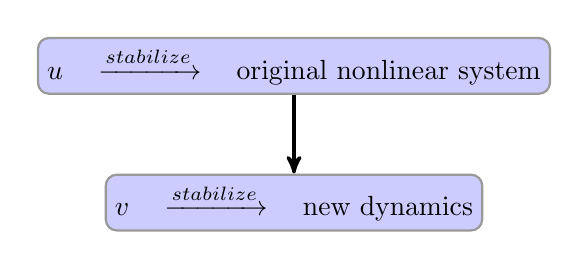
\begin{tikzpicture}[scale=0.5, auto, >=stealth']
      \matrix[ampersand replacement=\&, row sep=1cm, column sep=0.8cm]{
      \node [block] (origin) {$u \quad \xrightarrow{stabilize} \quad \text{original nonlinear system}$}; \\
      \node [block] (new) {$v \quad \xrightarrow{stabilize} \quad \text{new dynamics}$};\\
      };
      \draw [connector, very thick] ($(origin.south)$) --node{} (new);
    \end{tikzpicture}
    \end{figure}
  \end{frame}


\begin{frame}{Input-State Linearization, ctd'}
      The \textbf{closed-loop system} under the above control law is represented in the block diagram in Figure \ref{block}.
  \begin{figure}
  \centering
      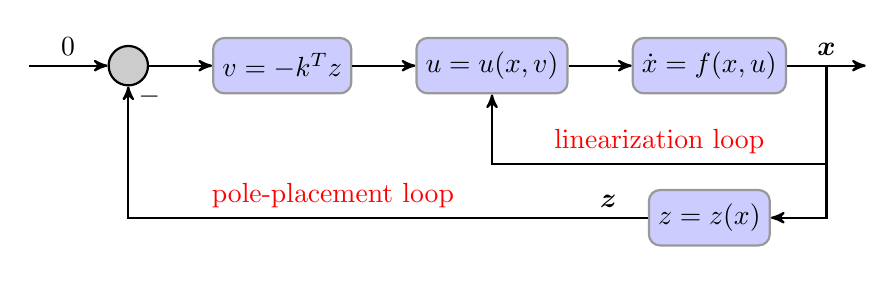
\begin{tikzpicture}[scale=0.5, auto, >=stealth']
      \matrix[ampersand replacement=\&, row sep=0.4cm, column sep=0.8cm]{

        \node[sum] (add) {};\&
        \node[block] (v) {$v=-k^{T}z$};\&
        \node[block] (u) {$u=u(x, v)$};\&
        \node[block] (dotx) {$\dot{x}=f(x,u)$}; \\
        \& \& \& \\
        \& \& \& \\
        \& \& \&
        \node[block] (z) {$z=z(x)$}; \\
        };

        %draw the lines
        \draw [connector, thick] ($(add.west)+(-2cm, 0cm)$) --node{0} ($(add.west)+(0cm, 0cm)$);
        \draw [connector, thick] ($(add.east)$) --node{} (v);
        \draw [connector, thick] ($(v.east)$) --node{} (u);
        \draw [connector, thick] ($(u.east)$) --node{} (dotx);
        \draw [connector, thick] ($(dotx.east)$) --node[above]{\vec{x}} ($(dotx.east)+(2cm, 0cm)$);
        \draw [connector, thick] ($(dotx.east)+(1cm, 0cm)$) |- ($(z.east)$);

        %for control the position of word, we can divide a line into segments!
        \draw [connector, thick] ($(z.west)$) -- node [above] {\vec{z}} ($(z.west)+(-2cm, 0cm)$) -- node [near end,above] {\textcolor{red}{ pole-placement loop}} ($(z.west)+(-10cm, 0cm)$) -| ($(add.south)+(0cm,-1cm)$) -- node [near end,right] {$-$} (add);
        \draw [connector, thick] ($(dotx.east)+(1cm, -2.5cm)$) -| node [near start,above] {\textcolor{red}{linearization loop}} (u);
      \end{tikzpicture}
  \caption{Input-State Linearization}
  \label{block}
  \end{figure}
\end{frame}


\begin{frame}{Remarks}
    A number of remarks can be made about the above control law:
    \begin{itemize}
      \item The result, though valid in a \textbf{large region} of the state space, is not global.($x_{1}=(\pi/4 + k\pi/2), k=1,2,\dots$)
      \item In order to implement the control law, ($z_{1}, z_{2}$) \textbf{must be available}. ~If they are not physically meaningful or cannot be measured directly, the \textbf{original state} \vec{x} must be measured and used to compute them.
      \item In general, we rely on the system model both for the \textbf{controller design} and for the \textbf{computation of} $\textbf{z}$.
    \end{itemize}
\end{frame}


%====================================================
\section{4. Input-Output Linearization}


\begin{frame}{Input-Output Linearization}
Consider the \textbf{tracking control problem}, and the system
    \begin{equation}\label{tracking-control}
      \begin{aligned}
        \dot{\vec{x}} &= \vec{f}(\vec{x}, u) \\
        y &= h(\vec{x})
      \end{aligned}
    \end{equation}
The idea below constitutes the \textbf{intuitive basis} for the so-called \textbf{input-output linearization} approach to nonlinear control design:
    \begin{enumerate}
      \item \textcolor{red}{Objective} : make the output $y(t)$ track a desired trajectory $y_{d}(t)$ while keeping the whole state bounded.
      \item \textcolor{red}{Difficulty} : output $y$ is only indirectly related to the input $u$.
      \item \textcolor{red}{Try} : if we can find a direct and simple relation between the system output $y$ and the control input $u$ ?
    \end{enumerate}
\end{frame}


\begin{frame}{Example}
Consider the third-order system:
    \begin{equation}\label{third-order}
      \begin{aligned}
        \dot{x}_{1} &= \sin x_{2}+(x_{2}+1)x_{3} \\
        \dot{x}_{2} &= x_{1}^{5}+x_{3} \\
        \dot{x}_{3} &= x_{1}^{2}+u \\
        y &= x_{1}
      \end{aligned}
    \end{equation}
We find:
    $$
    \dot{y}=\dot{x}_{1}=\sin x_{2}+\left(x_{2}+1\right) x_{3}
    $$
    \begin{equation}\label{double}
      \ddot{y}=\left(x_{2}+1\right) u+f_{1}(x)
    \end{equation}
where $f_{1}(x)$ is a function of the state defined by
    \begin{equation}\label{f1x}
        f_{1}(x)=\left(x_{1}^{5}+x_{3}\right)\left(x_{3}+\cos x_{2}\right)+\left(x_{2}+1\right) x_{1}^{2}
    \end{equation}
\end{frame}


\begin{frame}{Example,ctd'}
    Clearly, (\ref{double}) represents an \textbf{explicit relationship} between $y$ and $u$.  If we choose the control input to be in the form
    $$
         \ddot{y}=\left(x_{2}+1\right) u+f_{1}(x) \quad \xrightarrow{ {\color{red}u=\frac{1}{x_{2}+1}\left(v-f_{1}\right)}} \quad \underbrace{\ddot{y} = v}_{linear~double-integrator}
    $$
   % $$
%       {\color{red}u=\frac{1}{x_{2}+1}\left(v-f_{1}\right)} \quad \xrightarrow[becomes]{E.q.(\ref{double})} \quad \underbrace{\ddot{y} = v}_{linear~double-integrator}
%    $$
Choosing $v$ as
\begin{equation}\label{choose-v}
  v = \ddot{y}_{d}-k_{1}e-k_{2}\dot{e}
\end{equation}
where $e=y(t)-y_{d}(t)$ be the \textbf{tracking error}, and $k_{1}, k_{2} > 0$.\\
So, the tracking error of the closed loop system is given by
$$
\ddot{e}+k_{2} \dot{e}+k_{1} e = 0
$$
which represents an \textbf{exponentially stable} error dynamics.
\end{frame}



%========================================================
\section{5. Mathematical Tools}

\begin{frame}{Introduction}
Every vector function \vec{f} corresponds a field of vectors in an $n$-dimensional space
$$
\text{A \textbf{vector function}}~\vec{f}:\mathbb{R}^{n}\rightarrow \mathbb{R}^{n} \quad \xrightarrow[geometry]{differential} \quad \text{A \textbf{vector field} in}~\mathbb{R}^{n}
$$

\begin{itemize}
  \item given a smooth scalar function $h(\vec{x})$ of the state \vec{x}, the gradient of $h$ is denoted by $\nabla h$
      $$
      {\color{red}\nabla h = \frac{\partial h}{\partial \vec{x}}}, \quad (\nabla h)_{j} = \frac{\partial h}{\partial x_{j}}
      $$
  \item given a vector field $\vec{f}(\vec{x})$, the Jacobian of \vec{f} if denoted by $\nabla \vec{f}$
      $$
      {\color{red}\nabla f = \frac{\partial \vec{f}}{\partial \vec{x}}}, \quad (\nabla \vec{f})_{ij} = \frac{\partial f_{i}}{\partial x_{j}}
      $$
\end{itemize}
\end{frame}


\begin{frame}{Lie Derivatives}
    \newtheorem{myDef}{Definition}
    \begin{myDef}
        Let $h : \mathbb{R}^{n} \rightarrow \mathbb{R}$ be a smooth scalar function, and $\vec{f} : \mathbb{R}^{n} \rightarrow \mathbb{R}^{n}$ be a smooth vector field on $\mathbb{R}^{n}$, then the \underline{Lie derivative of $h$ with}
        \underline{respect to \vec{f}} is a scalar function defined by {\color{red} $L_{\vec{f}}h = \nabla h ~\vec{f}$}.
    \end{myDef}

    The Lie derivative $L_{\vec{f}}h$ is simply the \textbf{directional derivative} of $h$ \textbf{along the direction of the vector \vec{f}}.
    \begin{itemize}
      \item $L_{\vec{f}}^{0}h = h$
      \item $L_{\vec{f}}^{i}h = L_{\vec{f}}(L_{\vec{f}}^{i-1}h) = \nabla(L_{\vec{f}}^{i-1}h )\vec{f}$
      \item $L_{\vec{g}}L_{\vec{f}}h = \nabla(L_{\vec{f}}h)g $
    \end{itemize}

\end{frame}

\begin{frame}{Example}
    One can easily see the relevance of Lie derivatives to dynamic systems by considering the following single-output system
    $$
    \begin{array}{l}{\dot{\mathbf{x}}=\mathbf{f}(\mathbf{x})} \\ {y=h(\mathbf{x})}\end{array}
    $$
    The derivatives of the output are
    $$
    \begin{array}{l}{\dot{y}=\frac{\partial h}{\partial \mathbf{x}} \dot{\mathbf{x}}=L_{\mathbf{f}} h} \\ \\
    {\ddot{y}=\frac{\partial\left[L_{\mathbf{f}} h\right]}{\partial \mathbf{x}} \dot{\mathbf{x}} = L_{\mathbf{f}}(L_{\mathbf{f}}h) = L_{\mathbf{f}}^{2} h}\end{array}
    $$
    and so on.
\end{frame}


\begin{frame}{Lie Brackets}
    \begin{myDef}
        Let \vec{f} and \vec{g} be two vector fields on $\mathbb{R}^{n}$. The \underline{Lie bracket of \vec{f}}
        \underline{and \vec{g}} is a third vector field defined by
        $$
        [\vec{f}, \vec{g}] = \nabla \vec{g} \vec{f} - \nabla \vec{f} \vec{g} = ad_{\vec{f}}\vec{g}
        $$
    \end{myDef}
    \begin{itemize}
      \item $ad_{\vec{f}}^{0}\vec{g} = \vec{g}$
      \item $ad_{\vec{f}}^{2}\vec{g} = [\vec{f}, [\vec{f}, \vec{g}]]$
      \item $ad_{\vec{f}}^{i}\vec{g} = [\vec{f}, ad_{\vec{f}}^{i-1}\vec{g}]$
    \end{itemize}
\end{frame}


\begin{frame}{An Example}
    \begin{figure}
      \centering
      \includegraphics[width=11cm]{image/example6-7.pdf}
      %\caption{}\label{}
    \end{figure}
\end{frame}


\begin{frame}{Properties of Lie Brackets}
    \textbf{\large Lemma}\quad Lie brackets have the following properties
    \begin{itemize}
      \item {\color{red}Bilinearity}:
        $$
        \begin{array}{l}{\left[\alpha_{1} f_{1}+\alpha_{2} f_{2}, g\right]=\alpha_{1}\left[f_{1}, g\right]+\alpha_{2}\left[f_{2}, g\right]} \\ {\left[f, \alpha_{1} g_{1}+\alpha_{2} g_{2}\right]=\alpha_{1}\left[f, g_{1}\right]+\alpha_{2}\left[f, g_{2}\right]}\end{array}
        $$
        where \vec{f}, $\vec{f}_{1}$, $\vec{f}_{2}$, $\vec{g}$, $\vec{g}_{1}$ and $\vec{g}_{2}$ are smooth vector fields, and $\alpha_{1}$ and $\alpha_{2}$ are constant scalars.

      \item {\color{red}Skew-commutativity}:
      $$
      [\vec{f}, \vec{g}] = -[\vec{g}, \vec{f}]
      $$

      \item {\color{red}Jacobi identity}:
      $$
      L_{ad_{\vec{f}}\vec{g}}h = L_{\vec{f}} L_{\vec{g}} h - L_{\vec{g}} L_{\vec{f}} h
      $$
    \end{itemize}
\end{frame}


\begin{frame}{Diffeomorphisms And State Transformations}
    \begin{myDef}
        A function ~$\vec{\phi}$ : $\mathbb{R}^{n} \rightarrow \mathbb{R}^{n}$, defined in a region $\Omega$, is called a \underline{diffeomorphism} \footnote{https://en.wikipedia.org/wiki/Diffeomorphism} if it is smooth, and if its inverse $\vec{\phi} ^{-1}$ exists and is smooth.
    \end{myDef}

    \begin{itemize}
      \item Similar to the concept of \textbf{coordinate transformation}.
      \item Used to \textbf{transform a nonlinear system into another} system in terms of a new set of states.
    \end{itemize}
    $$
    \vec{\phi}(\vec{x}) \xrightarrow[whole~space~\mathbb{R}^{n}]{region~\Omega} \text{global diffeomorphism} \xrightarrow{rare} \text{local diffeomorphism}\footnote{Finite neighborhood of a given point.}
    $$
\end{frame}


\begin{frame}{Diffeomorphisms And State Transformations, ctd'}
    Given a nonlinear function $\vec{\phi} (\vec{x})$, check \textbf{local diffeomorphism} by using the following lemma:

    \begin{myLemma} \label{lemma1}
        Let $\vec{\phi} (\vec{x})$ be a smooth function defined in a region $\Omega$ in $\mathbb{R}^{n}$. If the {\color{red}Jacobian matrix} ~$\nabla \vec{\phi}$ is {\color{red}non-singular} at a point $\vec{x}=\vec{x}_{0}$ of $\Omega$, then $\vec{\phi}(\vec{x})$ defines a \textbf{local diffeomorphism} in a subregion of $\Omega$.
    \end{myLemma}
\end{frame}


\begin{frame}{Diffeomorphisms And State Transformations, ctd'}
Consider the dynamic system described by
    $$
    \begin{array}{l}{\dot{\mathbf{x}}=\mathbf{f}(\mathbf{x})+\mathbf{g}(\mathbf{x}) u} \\ {y=h(\mathbf{x})}\end{array}
    $$
    and let a new set of states be defined by ~${\color{red}\vec{z}=\phi(\vec{x})}$~, Differentiation of ~$z$~ yields
    $$
    \dot{\mathbf{z}}=\frac{\partial \vec{\phi}}{\partial \mathbf{x}} \dot{\mathbf{x}}=\frac{\partial \vec{\phi}}{\partial \mathbf{x}}(\mathbf{f}(\mathbf{x})+\mathbf{g}(\mathbf{x}) u)
    $$
    One can easily write the new state-space representation as
    $$
    \begin{array}{l}{\dot{\vec{z}}=\vec{f}^{*}(\vec{z})+\vec{g}^{*}(\vec{z})u} \\ {y=h^{*}(\vec{z})}\end{array}
    $$
    where $\vec{x}=\vec{\phi}^{-1}(\vec{z})$ has been used, and the functions $\vec{f}^{*}$, $\vec{f}^{*}$ and $h^{*}$ are defined obviously.
\end{frame}


\begin{frame}{Example}
    \begin{figure}
      \centering
      \includegraphics[width=10cm]{image/ex6-8.pdf}
    \end{figure}
    \vspace{-10pt}
    $$
    \Omega = \{ (x_{1}, x_{2}), |x_{2}| < \frac{\pi}{2} \}
    $$
\end{frame}
\begin{frame}{Example}
    \begin{figure}
      \centering
      \includegraphics[width=10cm]{image/ex6-8.pdf}
    \end{figure}
    \vspace{-10pt}
    $$
    \Omega = \{ (x_{1}, x_{2}), |x_{2}| < \frac{\pi}{2} \}
    $$
    {\color{red}\large Question : how to calculates the $\vec{x}=\vec{\phi}^{-1}(\vec{z})$ ?}
\end{frame}


\begin{frame}{The Frobenius Theorem}
    The Frobenius theorem provides a \textbf{necessary and sufficient} condition for the \textbf{solvability} of a special class of \textbf{partial differential equations}\\
    Consider the set of first-order partial differential equations.
    \begin{equation}\label{partial-equation}
      \left\{ \begin{array}{c}
                \nabla h~\vec{f}=\frac{\partial h}{\partial x_{1}}f_{1}+\frac{\partial h}{\partial x_{2}}f_{2}+\frac{\partial h}{\partial x_{3}}f_{3}=0 \\
                \nabla h~\vec{g}=\frac{\partial h}{\partial x_{1}}g_{1}+\frac{\partial h}{\partial x_{2}}g_{2}+\frac{\partial h}{\partial x_{3}}g_{3}=0
              \end{array}\right.
    \end{equation}

    \begin{itemize}
      \item $f_{i}(x_{1},x_{2},x_{3}),~g_{i}(x_{1},x_{2},x_{3})(i=1,2,3)$, known, scalar functions.
      \item $h(x_{1},x_{2},x_{3})$, unknown.
    \end{itemize}
\end{frame}


\begin{frame}{The Frobenius Theorem, ctd'}
    Clearly, this set of partial differential equations is uniquely defined by the two vectors:
    $$
    \vec{f}=[f_{1}~f_{2}~f_{3}]^{T},\quad \vec{g}=[g_{1}~g_{2}~g_{3}]^{T}
    $$
    \vspace{-10pt}
    $$
    \exists ~h(x_{1},x_{2},x_{3}) \quad \xrightarrow{satisfied~E.q.(\ref{partial-equation})} \quad [\vec{f}, \vec{g}] ~is ~{\color{red}completely ~integrable}.
    $$

    {\color{red} Involutivity condition} on the vector fields $[\vec{f}, \vec{g}]$:\\
    E.q.(\ref{partial-equation}) has a solution $h(x_{1},x_{2},x_{3})$
    iff
    $\exists ~\alpha_{1}(x_{1},x_{2},x_{3})~,~\alpha_{2}(x_{1},x_{2},x_{3}) ~s.t.~[\vec{f},\vec{g}] = \alpha_{1}\vec{f}+\alpha_{2}\vec{g}$

    i.e., if the Lie bracket of \vec{f} and \vec{g} can be expressed as a linear combination of \vec{f} and \vec{g}.
\end{frame}




\end{document}










